\SourceLeaf{229}%
sich beweisen, dass solche immer in einem Planum liege.
\begin{center}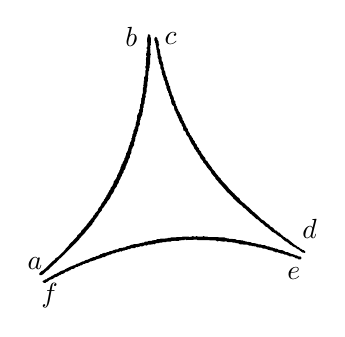
\begin{tikzpicture}[x=0.00543933cm,y=-0.00543933cm]
\fill[even odd rule] (663,563) -- (660,560) -- (657,561) -- (652,558) -- (649,558) -- (646,556) -- (638,554) -- (630,550) -- (626,550) -- (619,546) -- (610,545) -- (605,542) -- (601,542) -- (600,541) -- (598,541) -- (594,539) -- (591,539) -- (587,537) -- (583,537) -- (577,534) -- (571,534) -- (567,532) -- (562,532) -- (561,531) -- (558,531) -- (557,530) -- (554,530) -- (553,529) -- (548,529) -- (544,527) -- (535,526) -- (534,525) -- (531,525) -- (530,524) -- (527,524) -- (526,523) -- (521,523) -- (520,522) -- (512,522) -- (508,520) -- (493,519) -- (492,518) -- (488,518) -- (487,517) -- (484,517) -- (483,516) -- (469,516) -- (468,515) -- (444,515) -- (443,514) -- (436,514) -- (435,513) -- (433,513) -- (432,514) -- (420,514) -- (419,513) -- (417,513) -- (416,514) -- (411,514) -- (410,513) -- (408,513) -- (407,514) -- (404,514) -- (403,515) -- (401,515) -- (400,514) -- (385,514) -- (384,515) -- (358,516) -- (357,517) -- (351,517) -- (350,518) -- (345,518) -- (344,519) -- (333,519) -- (332,520) -- (325,520) -- (323,522) -- (318,522) -- (317,523) -- (314,523) -- (313,524) -- (306,524) -- (302,526) -- (297,526) -- (295,528) -- (290,528) -- (289,529) -- (283,530) -- (282,531) -- (270,532) -- (269,533) -- (266,533) -- (259,536) -- (253,537) -- (251,539) -- (247,539) -- (246,540) -- (237,541) -- (233,544) -- (228,544) -- (227,545) -- (224,545) -- (222,547) -- (220,547) -- (219,548) -- (215,548) -- (212,550) -- (209,550) -- (206,552) -- (201,552) -- (200,553) -- (198,553) -- (196,555) -- (193,555) -- (191,557) -- (187,559) -- (184,559) -- (180,562) -- (176,562) -- (173,564) -- (171,564) -- (163,568) -- (158,569) -- (154,572) -- (151,572) -- (141,577) -- (138,577) -- (136,579) -- (132,581) -- (129,581) -- (127,583) -- (123,584) -- (111,590) -- (109,592) -- (102,594) -- (98,596) -- (96,598) -- (94,598) -- (90,601) -- (86,602) -- (82,605) -- (80,605) -- (77,608) -- (75,608) -- (73,610) -- (70,611) -- (67,614) -- (64,614) -- (62,616) -- (59,617) -- (58,618) -- (58,620) -- (61,622) -- (65,622) -- (67,620) -- (70,619) -- (73,616) -- (77,614) -- (79,614) -- (83,612) -- (85,610) -- (89,608) -- (91,608) -- (95,606) -- (97,604) -- (99,604) -- (101,602) -- (108,600) -- (112,596) -- (116,596) -- (120,593) -- (122,593) -- (125,590) -- (131,589) -- (136,585) -- (140,585) -- (142,583) -- (144,583) -- (146,581) -- (149,581) -- (153,578) -- (156,578) -- (159,576) -- (165,575) -- (169,572) -- (172,572) -- (173,571) -- (181,569) -- (184,567) -- (195,564) -- (198,562) -- (202,562) -- (209,558) -- (211,558) -- (214,556) -- (217,556) -- (222,553) -- (226,553) -- (227,552) -- (229,552) -- (231,550) -- (236,550) -- (239,548) -- (242,549) -- (245,547) -- (248,547) -- (252,545) -- (255,545) -- (258,543) -- (262,543) -- (265,541) -- (273,541) -- (277,538) -- (279,539) -- (281,538) -- (284,538) -- (286,536) -- (288,537) -- (291,537) -- (297,534) -- (301,535) -- (304,533) -- (311,533) -- (312,532) -- (315,532) -- (316,531) -- (319,532) -- (324,529) -- (330,529) -- (331,528) -- (337,528) -- (338,527) -- (346,527) -- (347,526) -- (357,526) -- (360,524) -- (366,524) -- (367,523) -- (369,524) -- (376,524) -- (377,523) -- (381,523) -- (382,522) -- (389,522) -- (390,521) -- (393,521) -- (394,522) -- (419,521) -- (420,522) -- (448,522) -- (449,523) -- (463,523) -- (466,525) -- (468,525) -- (469,524) -- (473,524) -- (474,525) -- (478,525) -- (479,526) -- (487,525) -- (491,527) -- (501,527) -- (502,528) -- (508,528) -- (509,529) -- (513,529) -- (514,530) -- (516,530) -- (519,532) -- (537,533) -- (541,535) -- (546,535) -- (547,536) -- (557,537) -- (559,539) -- (570,540) -- (573,542) -- (579,542) -- (580,543) -- (583,543) -- (585,545) -- (596,547) -- (598,549) -- (600,549) -- (603,551) -- (607,550) -- (610,552) -- (612,552) -- (616,554) -- (620,554) -- (623,556) -- (628,556) -- (630,558) -- (632,558) -- (635,560) -- (641,560) -- (648,563) -- (650,565) -- (654,565) -- (656,567) -- (661,567) -- (663,565) -- cycle
(322,47) -- (319,51) -- (319,55) -- (321,58) -- (321,61) -- (322,62) -- (322,66) -- (323,67) -- (323,71) -- (324,72) -- (324,77) -- (325,78) -- (325,83) -- (326,84) -- (327,96) -- (329,100) -- (329,105) -- (330,106) -- (330,109) -- (333,113) -- (333,120) -- (336,125) -- (336,131) -- (337,132) -- (337,135) -- (339,138) -- (339,141) -- (341,143) -- (341,147) -- (344,152) -- (345,159) -- (347,162) -- (347,167) -- (349,169) -- (349,172) -- (351,174) -- (351,177) -- (353,179) -- (353,183) -- (356,188) -- (356,191) -- (358,194) -- (358,199) -- (359,200) -- (359,202) -- (361,206) -- (365,210) -- (366,218) -- (369,222) -- (369,224) -- (372,229) -- (372,231) -- (374,233) -- (374,236) -- (376,238) -- (377,242) -- (380,248) -- (383,251) -- (383,254) -- (386,258) -- (387,266) -- (389,266) -- (392,269) -- (394,276) -- (400,283) -- (400,285) -- (406,297) -- (410,302) -- (413,309) -- (416,312) -- (416,314) -- (420,318) -- (420,320) -- (424,324) -- (427,331) -- (433,338) -- (433,340) -- (438,345) -- (443,353) -- (451,362) -- (453,367) -- (462,377) -- (462,379) -- (469,386) -- (469,387) -- (476,394) -- (476,395) -- (477,395) -- (478,397) -- (480,398) -- (480,399) -- (488,408) -- (488,409) -- (490,411) -- (491,411) -- (503,423) -- (503,424) -- (518,438) -- (523,441) -- (528,447) -- (531,448) -- (534,451) -- (534,452) -- (536,453) -- (544,461) -- (545,461) -- (550,466) -- (551,466) -- (558,473) -- (561,474) -- (569,482) -- (572,483) -- (580,491) -- (582,491) -- (595,503) -- (598,504) -- (600,506) -- (602,506) -- (607,511) -- (608,511) -- (611,514) -- (613,514) -- (625,525) -- (627,525) -- (629,527) -- (630,527) -- (638,534) -- (640,534) -- (643,537) -- (650,540) -- (653,543) -- (655,543) -- (665,551) -- (671,552) -- (672,551) -- (672,549) -- (669,546) -- (665,545) -- (663,543) -- (660,542) -- (657,539) -- (654,538) -- (651,535) -- (648,534) -- (630,519) -- (628,519) -- (624,515) -- (622,515) -- (617,510) -- (616,510) -- (612,505) -- (608,504) -- (605,500) -- (602,500) -- (596,493) -- (591,491) -- (587,486) -- (582,483) -- (576,477) -- (570,474) -- (558,462) -- (557,462) -- (552,457) -- (551,457) -- (538,444) -- (537,444) -- (529,436) -- (524,433) -- (519,428) -- (519,426) -- (515,422) -- (514,422) -- (507,415) -- (507,414) -- (505,413) -- (492,400) -- (492,399) -- (475,381) -- (474,378) -- (469,374) -- (469,373) -- (462,365) -- (461,362) -- (455,356) -- (453,352) -- (445,342) -- (444,339) -- (439,335) -- (438,330) -- (433,325) -- (433,324) -- (429,319) -- (428,315) -- (424,311) -- (424,308) -- (419,303) -- (418,299) -- (414,295) -- (414,292) -- (409,286) -- (409,284) -- (406,281) -- (406,279) -- (402,275) -- (402,273) -- (398,267) -- (397,262) -- (394,259) -- (394,257) -- (392,255) -- (392,253) -- (388,246) -- (388,244) -- (385,241) -- (385,238) -- (382,232) -- (382,230) -- (379,227) -- (379,225) -- (375,220) -- (375,218) -- (373,215) -- (372,210) -- (370,208) -- (370,206) -- (368,202) -- (368,198) -- (365,195) -- (364,188) -- (360,181) -- (359,175) -- (357,172) -- (357,169) -- (356,168) -- (356,163) -- (353,160) -- (353,156) -- (352,155) -- (351,150) -- (349,147) -- (349,142) -- (346,138) -- (344,127) -- (342,125) -- (342,121) -- (340,117) -- (340,111) -- (339,110) -- (339,107) -- (336,102) -- (336,95) -- (334,92) -- (334,89) -- (333,88) -- (332,77) -- (329,73) -- (329,68) -- (330,67) -- (330,64) -- (329,63) -- (329,58) -- (326,53) -- (326,50) -- (323,47) -- cycle
(307,41) -- (305,41) -- (304,42) -- (304,46) -- (303,47) -- (303,50) -- (302,51) -- (303,52) -- (302,53) -- (302,59) -- (303,60) -- (303,70) -- (301,72) -- (301,75) -- (303,77) -- (303,78) -- (301,80) -- (301,85) -- (300,86) -- (300,91) -- (301,92) -- (301,94) -- (300,95) -- (300,98) -- (299,99) -- (300,101) -- (300,107) -- (299,108) -- (300,114) -- (298,116) -- (298,120) -- (299,121) -- (299,125) -- (298,126) -- (298,137) -- (295,142) -- (295,146) -- (296,148) -- (294,150) -- (295,153) -- (294,154) -- (294,159) -- (293,160) -- (294,164) -- (292,166) -- (292,179) -- (291,180) -- (290,189) -- (288,192) -- (289,195) -- (288,196) -- (288,202) -- (286,205) -- (285,216) -- (283,218) -- (284,223) -- (282,225) -- (279,231) -- (279,237) -- (278,238) -- (279,241) -- (277,243) -- (277,246) -- (276,247) -- (276,250) -- (275,251) -- (275,256) -- (273,259) -- (273,262) -- (270,267) -- (270,272) -- (268,275) -- (267,283) -- (265,285) -- (266,288) -- (262,295) -- (262,299) -- (260,301) -- (257,313) -- (255,317) -- (253,319) -- (253,323) -- (252,324) -- (251,329) -- (249,331) -- (249,334) -- (245,341) -- (245,343) -- (242,346) -- (242,349) -- (240,352) -- (239,358) -- (237,360) -- (237,362) -- (232,371) -- (232,374) -- (230,376) -- (230,378) -- (228,380) -- (228,381) -- (225,384) -- (224,386) -- (224,389) -- (222,392) -- (222,394) -- (217,400) -- (216,404) -- (213,407) -- (213,409) -- (210,413) -- (210,415) -- (207,418) -- (207,420) -- (205,422) -- (204,425) -- (201,428) -- (201,430) -- (196,436) -- (193,443) -- (189,447) -- (187,451) -- (187,453) -- (180,460) -- (180,462) -- (176,466) -- (176,468) -- (170,474) -- (170,475) -- (166,479) -- (166,480) -- (160,487) -- (160,488) -- (148,501) -- (148,503) -- (139,511) -- (138,514) -- (130,522) -- (130,523) -- (121,531) -- (118,536) -- (111,543) -- (111,544) -- (107,548) -- (107,549) -- (105,551) -- (104,551) -- (93,562) -- (89,564) -- (87,566) -- (87,567) -- (84,570) -- (83,570) -- (64,589) -- (63,589) -- (59,593) -- (55,595) -- (50,600) -- (50,603) -- (51,604) -- (55,604) -- (56,603) -- (58,603) -- (68,593) -- (70,593) -- (78,584) -- (79,584) -- (87,576) -- (88,576) -- (98,565) -- (99,565) -- (107,557) -- (108,557) -- (109,555) -- (134,530) -- (136,529) -- (136,528) -- (144,520) -- (144,519) -- (148,515) -- (148,514) -- (158,504) -- (158,503) -- (167,493) -- (167,492) -- (171,489) -- (171,488) -- (174,485) -- (175,482) -- (179,478) -- (179,476) -- (189,463) -- (189,461) -- (196,453) -- (197,449) -- (201,445) -- (203,441) -- (208,435) -- (209,432) -- (215,425) -- (219,416) -- (222,413) -- (225,407) -- (226,403) -- (231,397) -- (232,393) -- (234,391) -- (236,387) -- (236,385) -- (240,378) -- (240,376) -- (243,372) -- (244,368) -- (247,364) -- (247,360) -- (250,357) -- (252,353) -- (252,350) -- (254,347) -- (254,345) -- (257,340) -- (259,333) -- (262,329) -- (262,324) -- (265,319) -- (266,310) -- (268,307) -- (268,305) -- (270,303) -- (272,299) -- (272,293) -- (274,290) -- (275,281) -- (277,278) -- (277,275) -- (279,272) -- (279,269) -- (281,266) -- (282,257) -- (285,252) -- (285,249) -- (284,248) -- (285,246) -- (285,243) -- (287,241) -- (287,237) -- (291,229) -- (291,224) -- (292,223) -- (292,219) -- (293,218) -- (292,214) -- (294,212) -- (294,206) -- (296,203) -- (297,191) -- (299,187) -- (298,182) -- (300,180) -- (300,177) -- (301,176) -- (301,166) -- (302,165) -- (302,162) -- (303,161) -- (303,152) -- (304,151) -- (304,145) -- (305,144) -- (304,142) -- (304,138) -- (305,137) -- (305,128) -- (307,125) -- (307,120) -- (308,119) -- (308,112) -- (309,111) -- (309,96) -- (310,95) -- (310,90) -- (311,89) -- (311,87) -- (310,86) -- (310,77) -- (309,76) -- (309,74) -- (310,73) -- (309,68) -- (311,66) -- (311,64) -- (310,63) -- (311,61) -- (311,49) -- (310,48) -- (310,44) -- cycle;
\node[inner sep=0pt] at (265,48) {$b$};
\node[inner sep=0pt] at (357,50) {$c$};
\node[inner sep=0pt] at (40,578) {$a$};
\node[inner sep=0pt] at (74,653) {$f$};
\node[inner sep=0pt] at (682,497) {$d$};
\node[inner sep=0pt] at (645,600) {$e$};
\end{tikzpicture}
\end{center}
II. Derjenige Theil des Planums, welcher \textls{zwischen}\HistoricalNote{*)}{*)}{Bei einer vollständigen Durchführung müssen solche Worte, wie »zwischen«, auch erst auf klare \textls{Begriffe} gebracht werden, was sehr gut angeht, was ich aber nirgends geleistet finde.} den drei Geraden $ab$, $cd$, $ef$ liegt, hat eine bestimmte endliche Area: sie heisse $t$.

\Needspace{20\baselineskip}
III. Indem zwei Geraden $ab$, $ac$ sich in $a$ unter dem Winkel $\varphi$ schneiden, möge eine dritte Gerade $de$ so beschaffen sein, dass $ab\TripleParallel ed$, $ac\TripleParallel de$: es liegt dann auch $de$ mit $ab$ und $ac$ in Einem Planum, und die Area der Fläche zwischen diesen Geraden ist endlich, und nur von dem Winkel $\varphi$ abhängig; offenbar bilden in $S$ $de$ und $bac$ nur Eine gerade Linie, wenn $\varphi=180^{0}$ ist, und folglich verschwindet der Werth jener Area mit $180^{0}-\varphi$: man setze also allgemein die Area $=f(180^{0}-\varphi)$, wo $f$ ein Functionalzeichen bezeichnet.
\begin{center}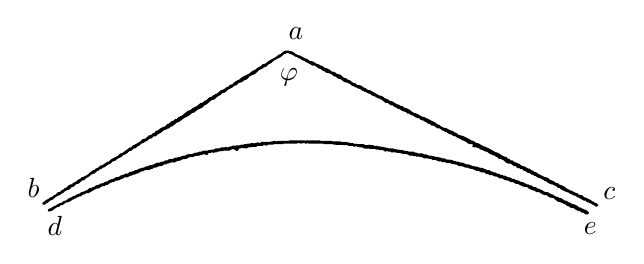
\begin{tikzpicture}[x=0.00691489cm,y=-0.00691489cm]
\fill[even odd rule] (62,365) -- (62,366) -- (64,368) -- (71,366) -- (74,363) -- (79,360) -- (83,359) -- (86,356) -- (89,356) -- (96,351) -- (99,351) -- (105,348) -- (107,346) -- (109,346) -- (111,344) -- (113,344) -- (115,342) -- (117,342) -- (120,340) -- (123,340) -- (126,337) -- (128,337) -- (133,334) -- (137,334) -- (151,326) -- (157,325) -- (159,323) -- (163,321) -- (167,321) -- (169,319) -- (172,319) -- (174,317) -- (180,314) -- (183,314) -- (187,311) -- (191,311) -- (192,310) -- (194,310) -- (197,308) -- (199,308) -- (203,305) -- (208,305) -- (214,302) -- (216,302) -- (219,300) -- (222,300) -- (225,298) -- (227,298) -- (234,294) -- (237,294) -- (240,292) -- (250,291) -- (251,290) -- (255,289) -- (257,287) -- (261,287) -- (265,285) -- (272,284) -- (276,281) -- (280,281) -- (281,280) -- (283,280) -- (287,278) -- (290,278) -- (291,277) -- (294,278) -- (300,275) -- (306,274) -- (309,272) -- (317,271) -- (322,268) -- (329,268) -- (332,266) -- (341,265) -- (342,264) -- (345,264) -- (346,263) -- (352,263) -- (353,264) -- (355,264) -- (358,260) -- (362,260) -- (363,259) -- (367,260) -- (368,259) -- (372,259) -- (373,258) -- (377,258) -- (378,257) -- (384,257) -- (385,256) -- (396,256) -- (401,253) -- (403,253) -- (410,257) -- (414,252) -- (417,252) -- (418,251) -- (428,252) -- (430,250) -- (435,250) -- (436,249) -- (445,249) -- (448,247) -- (457,247) -- (458,246) -- (461,246) -- (463,247) -- (467,245) -- (476,245) -- (477,244) -- (494,244) -- (495,243) -- (520,243) -- (521,242) -- (525,242) -- (526,243) -- (534,242) -- (535,243) -- (538,243) -- (540,242) -- (541,243) -- (568,243) -- (569,244) -- (586,244) -- (587,245) -- (613,246) -- (614,247) -- (621,247) -- (625,249) -- (627,248) -- (630,248) -- (631,249) -- (634,249) -- (635,250) -- (640,250) -- (643,252) -- (664,253) -- (665,254) -- (670,254) -- (671,255) -- (678,255) -- (682,258) -- (684,257) -- (687,257) -- (688,258) -- (692,258) -- (693,259) -- (702,259) -- (703,260) -- (709,260) -- (710,261) -- (713,261) -- (714,262) -- (720,262) -- (721,263) -- (724,263) -- (726,265) -- (732,265) -- (733,266) -- (738,266) -- (739,267) -- (745,267) -- (746,268) -- (750,268) -- (753,270) -- (761,270) -- (762,271) -- (765,271) -- (769,273) -- (774,273) -- (781,276) -- (784,275) -- (786,277) -- (792,277) -- (795,279) -- (799,279) -- (801,278) -- (803,280) -- (814,282) -- (816,284) -- (825,285) -- (829,287) -- (833,287) -- (837,289) -- (844,290) -- (846,292) -- (848,292) -- (849,293) -- (853,293) -- (859,296) -- (864,296) -- (868,299) -- (871,299) -- (874,301) -- (879,301) -- (882,303) -- (888,304) -- (892,307) -- (897,307) -- (902,310) -- (908,311) -- (913,314) -- (917,314) -- (922,317) -- (925,317) -- (935,322) -- (943,323) -- (945,325) -- (953,329) -- (955,329) -- (960,332) -- (965,332) -- (967,334) -- (973,337) -- (979,338) -- (984,342) -- (991,343) -- (998,349) -- (1000,350) -- (1003,350) -- (1006,352) -- (1008,352) -- (1010,354) -- (1012,354) -- (1017,358) -- (1019,358) -- (1023,361) -- (1029,362) -- (1031,364) -- (1037,367) -- (1040,367) -- (1043,370) -- (1046,370) -- (1050,373) -- (1054,373) -- (1056,371) -- (1056,369) -- (1051,365) -- (1049,365) -- (1047,363) -- (1045,363) -- (1040,360) -- (1038,360) -- (1036,358) -- (1030,355) -- (1023,353) -- (1021,351) -- (1019,351) -- (1015,348) -- (1012,348) -- (1005,343) -- (1002,343) -- (999,341) -- (997,341) -- (993,339) -- (991,337) -- (987,336) -- (980,332) -- (976,332) -- (972,330) -- (970,328) -- (968,328) -- (965,326) -- (962,326) -- (960,324) -- (958,323) -- (955,323) -- (951,320) -- (948,320) -- (945,318) -- (943,318) -- (935,314) -- (932,314) -- (927,311) -- (922,310) -- (919,308) -- (916,308) -- (911,305) -- (908,305) -- (902,302) -- (899,302) -- (898,301) -- (893,300) -- (890,298) -- (887,298) -- (884,296) -- (881,296) -- (878,294) -- (876,294) -- (874,292) -- (869,292) -- (866,290) -- (864,290) -- (862,288) -- (854,287) -- (853,286) -- (850,286) -- (849,285) -- (845,285) -- (844,284) -- (842,284) -- (835,281) -- (831,281) -- (824,278) -- (820,278) -- (816,276) -- (812,276) -- (811,275) -- (808,275) -- (804,273) -- (793,272) -- (791,270) -- (786,270) -- (785,269) -- (782,269) -- (781,268) -- (776,268) -- (775,267) -- (772,267) -- (771,266) -- (768,266) -- (767,265) -- (762,265) -- (761,264) -- (759,264) -- (758,263) -- (754,263) -- (750,261) -- (742,261) -- (741,260) -- (735,259) -- (734,258) -- (725,258) -- (724,257) -- (720,257) -- (719,256) -- (715,256) -- (714,255) -- (709,255) -- (708,254) -- (703,254) -- (702,253) -- (698,253) -- (697,252) -- (688,252) -- (687,251) -- (684,251) -- (683,250) -- (680,250) -- (679,249) -- (674,249) -- (673,248) -- (669,248) -- (668,247) -- (661,247) -- (660,246) -- (655,246) -- (654,245) -- (652,245) -- (651,246) -- (646,246) -- (642,244) -- (630,244) -- (629,243) -- (626,244) -- (623,242) -- (617,242) -- (616,241) -- (612,241) -- (611,240) -- (601,240) -- (600,239) -- (585,239) -- (584,238) -- (563,238) -- (562,237) -- (556,237) -- (555,238) -- (553,237) -- (544,237) -- (543,238) -- (541,237) -- (536,237) -- (535,238) -- (533,237) -- (506,237) -- (505,238) -- (484,238) -- (483,239) -- (477,238) -- (476,239) -- (472,239) -- (471,240) -- (454,240) -- (452,242) -- (450,242) -- (449,241) -- (446,241) -- (445,242) -- (442,242) -- (441,243) -- (439,242) -- (435,242) -- (434,243) -- (429,243) -- (428,244) -- (423,244) -- (422,245) -- (417,245) -- (416,246) -- (401,247) -- (400,248) -- (394,249) -- (393,250) -- (391,250) -- (390,249) -- (388,249) -- (387,250) -- (381,250) -- (377,252) -- (370,252) -- (367,254) -- (362,254) -- (361,255) -- (357,255) -- (356,256) -- (348,256) -- (344,258) -- (340,258) -- (339,259) -- (332,260) -- (328,262) -- (317,263) -- (315,265) -- (311,265) -- (304,268) -- (301,268) -- (300,269) -- (296,269) -- (292,271) -- (284,272) -- (282,274) -- (278,274) -- (275,276) -- (271,276) -- (268,278) -- (263,278) -- (255,282) -- (249,283) -- (245,285) -- (242,285) -- (239,287) -- (236,287) -- (235,288) -- (230,289) -- (227,291) -- (222,292) -- (219,294) -- (213,295) -- (209,298) -- (205,298) -- (202,300) -- (195,302) -- (193,304) -- (187,305) -- (182,308) -- (177,309) -- (173,311) -- (171,313) -- (168,313) -- (163,316) -- (160,316) -- (155,319) -- (153,319) -- (149,321) -- (147,323) -- (145,323) -- (141,325) -- (138,325) -- (134,329) -- (132,329) -- (129,331) -- (124,332) -- (120,335) -- (114,337) -- (112,339) -- (109,339) -- (106,342) -- (104,342) -- (100,344) -- (95,348) -- (93,348) -- (89,350) -- (87,352) -- (85,352) -- (79,355) -- (77,357) -- (75,357) -- (73,359) -- (71,359) -- (69,361) -- (64,363) -- cycle
(52,352) -- (52,354) -- (53,355) -- (57,355) -- (59,353) -- (62,352) -- (66,348) -- (71,346) -- (78,340) -- (85,337) -- (88,334) -- (90,334) -- (94,330) -- (102,327) -- (106,323) -- (110,322) -- (115,317) -- (118,317) -- (125,311) -- (129,310) -- (133,306) -- (136,305) -- (142,300) -- (146,298) -- (148,298) -- (153,293) -- (155,293) -- (158,290) -- (160,290) -- (162,288) -- (167,286) -- (172,282) -- (177,280) -- (181,276) -- (187,274) -- (190,271) -- (198,267) -- (201,264) -- (206,262) -- (212,257) -- (216,256) -- (220,252) -- (223,252) -- (228,247) -- (230,247) -- (234,243) -- (238,242) -- (240,240) -- (246,237) -- (249,234) -- (252,234) -- (256,230) -- (260,230) -- (264,226) -- (270,223) -- (276,218) -- (278,218) -- (281,216) -- (285,215) -- (288,212) -- (291,211) -- (300,204) -- (302,204) -- (313,196) -- (321,192) -- (327,187) -- (331,186) -- (337,181) -- (346,177) -- (351,172) -- (354,171) -- (363,163) -- (368,162) -- (373,157) -- (374,157) -- (376,155) -- (378,155) -- (382,151) -- (388,149) -- (393,144) -- (401,140) -- (406,136) -- (409,136) -- (412,132) -- (419,130) -- (424,126) -- (426,126) -- (428,124) -- (429,124) -- (433,119) -- (435,119) -- (437,117) -- (439,117) -- (443,115) -- (449,109) -- (454,106) -- (456,106) -- (459,103) -- (463,102) -- (468,97) -- (473,95) -- (478,90) -- (490,84) -- (497,78) -- (499,78) -- (500,77) -- (505,77) -- (506,78) -- (510,79) -- (512,81) -- (514,81) -- (516,83) -- (520,84) -- (522,86) -- (526,87) -- (529,90) -- (531,90) -- (549,100) -- (553,100) -- (560,105) -- (564,106) -- (567,109) -- (570,110) -- (574,113) -- (580,114) -- (584,116) -- (587,119) -- (591,120) -- (596,124) -- (599,124) -- (607,130) -- (612,131) -- (618,134) -- (621,137) -- (623,137) -- (628,140) -- (630,140) -- (632,142) -- (634,142) -- (638,144) -- (640,146) -- (642,146) -- (644,148) -- (646,148) -- (651,151) -- (653,151) -- (660,156) -- (662,156) -- (669,160) -- (671,160) -- (673,162) -- (675,162) -- (681,167) -- (683,168) -- (686,168) -- (693,173) -- (696,173) -- (699,176) -- (703,177) -- (705,179) -- (709,180) -- (713,183) -- (720,185) -- (723,188) -- (726,188) -- (730,191) -- (732,191) -- (738,195) -- (745,197) -- (748,200) -- (750,200) -- (751,201) -- (753,201) -- (755,203) -- (757,203) -- (760,206) -- (764,207) -- (767,210) -- (771,210) -- (778,215) -- (782,215) -- (787,219) -- (789,219) -- (791,221) -- (795,222) -- (797,224) -- (801,226) -- (803,226) -- (807,229) -- (812,230) -- (814,232) -- (821,235) -- (823,237) -- (825,237) -- (831,240) -- (834,243) -- (836,243) -- (837,244) -- (842,244) -- (843,245) -- (842,249) -- (844,249) -- (845,250) -- (850,250) -- (851,251) -- (853,251) -- (857,254) -- (859,254) -- (867,258) -- (869,258) -- (873,261) -- (879,264) -- (883,265) -- (885,267) -- (888,268) -- (891,271) -- (894,271) -- (900,274) -- (904,278) -- (908,280) -- (913,280) -- (918,284) -- (921,284) -- (925,288) -- (928,288) -- (931,290) -- (934,290) -- (937,293) -- (939,293) -- (941,295) -- (945,297) -- (947,297) -- (951,300) -- (953,300) -- (957,303) -- (959,303) -- (963,306) -- (965,306) -- (973,310) -- (975,312) -- (977,312) -- (981,315) -- (987,318) -- (989,318) -- (997,322) -- (999,324) -- (1003,325) -- (1005,327) -- (1015,332) -- (1019,333) -- (1021,335) -- (1025,336) -- (1027,338) -- (1032,339) -- (1035,342) -- (1037,342) -- (1047,348) -- (1050,348) -- (1053,351) -- (1056,351) -- (1058,353) -- (1060,353) -- (1062,355) -- (1064,355) -- (1069,359) -- (1071,359) -- (1073,357) -- (1073,355) -- (1071,353) -- (1066,351) -- (1064,349) -- (1062,349) -- (1060,347) -- (1050,342) -- (1048,342) -- (1044,338) -- (1038,337) -- (1035,334) -- (1032,334) -- (1030,332) -- (1028,332) -- (1026,330) -- (1024,330) -- (1016,326) -- (1011,322) -- (1005,319) -- (1003,319) -- (1001,317) -- (997,315) -- (995,315) -- (993,313) -- (987,310) -- (985,310) -- (981,306) -- (974,304) -- (962,298) -- (960,296) -- (956,295) -- (954,293) -- (951,292) -- (947,289) -- (945,289) -- (938,285) -- (933,284) -- (928,280) -- (926,280) -- (924,278) -- (922,278) -- (918,276) -- (916,274) -- (913,274) -- (910,271) -- (908,271) -- (905,268) -- (901,267) -- (895,264) -- (893,262) -- (887,259) -- (885,259) -- (869,250) -- (867,250) -- (865,248) -- (862,248) -- (860,246) -- (858,246) -- (856,244) -- (852,242) -- (849,242) -- (847,240) -- (841,237) -- (839,237) -- (837,235) -- (825,229) -- (817,227) -- (812,223) -- (810,223) -- (808,221) -- (804,219) -- (802,219) -- (793,214) -- (790,214) -- (784,211) -- (782,209) -- (777,207) -- (775,205) -- (753,194) -- (751,194) -- (738,187) -- (736,187) -- (732,185) -- (727,181) -- (721,178) -- (719,178) -- (713,174) -- (711,174) -- (706,171) -- (704,171) -- (694,165) -- (691,165) -- (689,163) -- (680,159) -- (678,157) -- (674,155) -- (672,155) -- (654,145) -- (651,145) -- (644,140) -- (642,140) -- (640,138) -- (636,136) -- (630,135) -- (627,132) -- (624,132) -- (616,126) -- (614,126) -- (610,123) -- (606,122) -- (599,116) -- (596,116) -- (595,115) -- (593,115) -- (591,113) -- (587,111) -- (584,111) -- (581,108) -- (573,104) -- (571,104) -- (566,100) -- (564,100) -- (559,97) -- (557,97) -- (549,92) -- (543,91) -- (538,87) -- (536,87) -- (525,81) -- (523,81) -- (517,78) -- (512,74) -- (506,73) -- (505,72) -- (499,72) -- (495,74) -- (489,79) -- (487,79) -- (481,84) -- (468,91) -- (462,96) -- (457,97) -- (453,101) -- (447,104) -- (444,107) -- (439,109) -- (431,115) -- (419,121) -- (413,126) -- (411,126) -- (409,128) -- (406,129) -- (401,134) -- (397,135) -- (393,139) -- (391,139) -- (386,143) -- (380,145) -- (373,151) -- (371,151) -- (368,154) -- (366,154) -- (363,157) -- (359,158) -- (354,163) -- (351,164) -- (346,168) -- (343,168) -- (336,174) -- (328,178) -- (325,181) -- (319,183) -- (308,192) -- (306,192) -- (304,194) -- (302,194) -- (299,198) -- (296,198) -- (293,201) -- (289,202) -- (285,206) -- (282,207) -- (277,212) -- (275,212) -- (269,215) -- (264,219) -- (261,219) -- (258,223) -- (255,224) -- (252,227) -- (248,228) -- (241,234) -- (236,235) -- (230,241) -- (228,241) -- (226,243) -- (224,243) -- (222,245) -- (219,246) -- (215,250) -- (213,250) -- (198,261) -- (195,261) -- (190,266) -- (178,272) -- (174,276) -- (172,276) -- (165,281) -- (161,283) -- (159,283) -- (155,287) -- (150,289) -- (147,292) -- (145,292) -- (143,294) -- (142,294) -- (134,301) -- (128,304) -- (124,305) -- (121,308) -- (120,308) -- (112,314) -- (109,315) -- (106,318) -- (104,318) -- (100,320) -- (96,324) -- (93,325) -- (90,328) -- (88,328) -- (84,332) -- (81,332) -- (76,337) -- (73,338) -- (70,341) -- (66,342) -- (63,345) -- (60,346) -- cycle;
\node[inner sep=0pt] at (518,41) {$a$};
\node[inner sep=0pt] at (505,122) {$\varphi$};
\node[inner sep=0pt] at (36,325) {$b$};
\node[inner sep=0pt] at (75,395) {$d$};
\node[inner sep=0pt] at (1094,335) {$c$};
\node[inner sep=0pt] at (1059,400) {$e$};
\end{tikzpicture}
\end{center}

\Needspace{13\baselineskip}
IV. Lehrsatz. Es ist allgemein $f\varphi+f(180^{0}-\varphi)=t$.
\begin{center}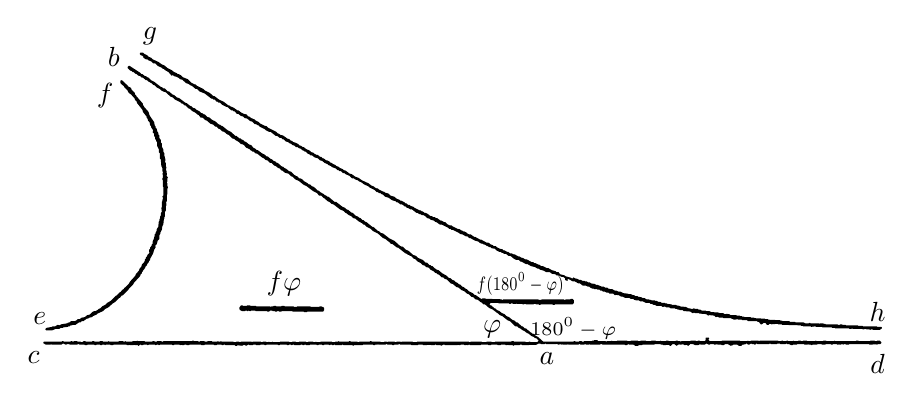
\begin{tikzpicture}[x=0.00648523cm,y=-0.00648523cm]
\fill[even odd rule] (430,571) -- (430,574) -- (431,576) -- (435,578) -- (441,578) -- (442,577) -- (444,577) -- (445,578) -- (447,578) -- (448,577) -- (450,578) -- (452,578) -- (453,577) -- (461,577) -- (462,578) -- (484,578) -- (485,579) -- (488,579) -- (490,577) -- (494,577) -- (495,578) -- (499,578) -- (500,579) -- (503,579) -- (504,578) -- (507,578) -- (508,579) -- (512,579) -- (513,578) -- (533,578) -- (534,579) -- (556,579) -- (557,580) -- (562,580) -- (563,579) -- (594,579) -- (596,576) -- (596,572) -- (594,570) -- (592,570) -- (591,569) -- (587,569) -- (586,570) -- (570,570) -- (569,569) -- (543,569) -- (542,570) -- (537,570) -- (536,569) -- (519,569) -- (518,568) -- (513,568) -- (512,569) -- (502,569) -- (501,568) -- (497,568) -- (496,569) -- (493,569) -- (491,570) -- (490,569) -- (463,569) -- (462,568) -- (452,568) -- (451,567) -- (445,567) -- (444,568) -- (437,568) -- (436,567) -- (433,567) -- cycle
(199,126) -- (197,127) -- (197,131) -- (198,133) -- (204,138) -- (204,139) -- (211,146) -- (212,149) -- (216,153) -- (217,153) -- (225,162) -- (225,164) -- (229,168) -- (229,170) -- (240,184) -- (241,188) -- (248,197) -- (248,199) -- (250,201) -- (251,205) -- (254,208) -- (255,214) -- (257,216) -- (257,218) -- (261,224) -- (260,228) -- (263,231) -- (263,235) -- (265,238) -- (265,241) -- (267,243) -- (267,245) -- (269,248) -- (269,255) -- (272,261) -- (272,267) -- (274,269) -- (274,279) -- (276,281) -- (277,294) -- (279,298) -- (279,304) -- (280,305) -- (280,308) -- (279,309) -- (280,311) -- (280,317) -- (279,318) -- (279,321) -- (280,322) -- (280,334) -- (281,335) -- (281,352) -- (279,354) -- (280,356) -- (280,359) -- (279,360) -- (279,363) -- (278,364) -- (278,375) -- (277,376) -- (278,383) -- (276,387) -- (276,391) -- (275,392) -- (274,398) -- (273,399) -- (273,402) -- (272,403) -- (271,413) -- (268,418) -- (268,421) -- (266,424) -- (266,426) -- (264,428) -- (264,432) -- (263,433) -- (263,435) -- (260,442) -- (260,446) -- (258,448) -- (258,450) -- (255,454) -- (255,456) -- (253,458) -- (253,462) -- (254,464) -- (250,468) -- (249,471) -- (247,473) -- (247,475) -- (245,477) -- (245,479) -- (243,483) -- (239,487) -- (238,491) -- (235,494) -- (233,499) -- (227,506) -- (226,509) -- (216,520) -- (213,525) -- (206,532) -- (205,532) -- (204,534) -- (202,536) -- (201,536) -- (197,541) -- (196,541) -- (189,548) -- (188,548) -- (178,558) -- (171,562) -- (167,566) -- (161,569) -- (157,573) -- (154,574) -- (152,576) -- (148,578) -- (146,578) -- (142,580) -- (137,585) -- (132,586) -- (127,590) -- (121,591) -- (117,594) -- (113,594) -- (111,596) -- (107,598) -- (100,598) -- (98,600) -- (94,601) -- (93,602) -- (81,604) -- (78,606) -- (74,605) -- (69,608) -- (64,608) -- (63,609) -- (52,611) -- (50,613) -- (50,614) -- (52,616) -- (63,616) -- (70,613) -- (77,613) -- (80,611) -- (84,611) -- (85,610) -- (94,609) -- (95,608) -- (97,608) -- (99,606) -- (102,606) -- (103,605) -- (109,605) -- (116,600) -- (119,600) -- (121,598) -- (124,598) -- (131,593) -- (133,593) -- (136,591) -- (141,590) -- (143,588) -- (150,585) -- (152,583) -- (163,578) -- (167,574) -- (173,571) -- (182,563) -- (187,560) -- (195,552) -- (196,552) -- (199,548) -- (202,547) -- (213,536) -- (213,535) -- (221,527) -- (224,522) -- (236,509) -- (236,507) -- (239,504) -- (239,502) -- (241,500) -- (241,499) -- (245,494) -- (246,491) -- (249,488) -- (249,486) -- (252,483) -- (253,480) -- (255,478) -- (255,476) -- (261,465) -- (263,458) -- (266,453) -- (265,450) -- (268,447) -- (270,440) -- (273,437) -- (273,430) -- (275,427) -- (275,425) -- (278,419) -- (279,412) -- (281,408) -- (282,398) -- (283,397) -- (283,394) -- (284,393) -- (284,384) -- (286,381) -- (286,372) -- (287,371) -- (287,368) -- (286,366) -- (288,362) -- (288,350) -- (289,349) -- (289,338) -- (290,337) -- (290,335) -- (289,334) -- (289,328) -- (288,327) -- (288,325) -- (289,324) -- (289,318) -- (290,316) -- (287,313) -- (288,311) -- (287,303) -- (286,302) -- (287,296) -- (286,295) -- (286,288) -- (284,286) -- (285,284) -- (285,280) -- (284,279) -- (284,276) -- (283,275) -- (283,269) -- (281,266) -- (281,262) -- (278,256) -- (278,250) -- (276,248) -- (276,243) -- (273,239) -- (273,234) -- (271,232) -- (271,229) -- (269,226) -- (268,221) -- (266,219) -- (266,217) -- (264,214) -- (263,208) -- (254,195) -- (252,188) -- (244,179) -- (241,174) -- (241,172) -- (228,157) -- (228,156) -- (225,153) -- (225,151) -- (219,145) -- (218,142) -- (216,140) -- (213,139) -- (209,134) -- (208,134) -- (201,127) -- cycle
(46,639) -- (46,641) -- (51,644) -- (60,644) -- (61,643) -- (63,644) -- (81,644) -- (84,642) -- (86,642) -- (90,644) -- (92,643) -- (97,643) -- (98,644) -- (112,644) -- (113,643) -- (116,643) -- (117,644) -- (127,644) -- (128,645) -- (131,645) -- (132,644) -- (146,644) -- (147,645) -- (149,645) -- (150,644) -- (157,644) -- (158,645) -- (160,645) -- (161,644) -- (166,644) -- (167,645) -- (168,644) -- (177,644) -- (178,645) -- (182,645) -- (183,644) -- (209,644) -- (210,645) -- (213,645) -- (215,644) -- (216,645) -- (222,645) -- (224,644) -- (225,645) -- (231,645) -- (232,646) -- (233,646) -- (235,644) -- (237,644) -- (238,645) -- (241,645) -- (242,644) -- (249,644) -- (250,645) -- (252,644) -- (265,644) -- (266,645) -- (268,644) -- (271,644) -- (272,645) -- (274,644) -- (298,644) -- (299,645) -- (301,645) -- (302,644) -- (313,644) -- (314,645) -- (316,644) -- (318,645) -- (321,645) -- (322,644) -- (326,644) -- (327,645) -- (331,645) -- (332,644) -- (355,644) -- (356,645) -- (361,645) -- (362,644) -- (380,644) -- (381,645) -- (385,645) -- (386,644) -- (395,644) -- (396,645) -- (398,645) -- (399,644) -- (402,644) -- (403,645) -- (421,645) -- (422,646) -- (425,646) -- (426,645) -- (435,646) -- (439,644) -- (443,646) -- (447,644) -- (449,644) -- (450,645) -- (456,645) -- (457,644) -- (462,644) -- (463,645) -- (470,645) -- (471,644) -- (479,644) -- (480,645) -- (482,645) -- (483,644) -- (505,644) -- (506,645) -- (508,645) -- (509,644) -- (523,644) -- (524,645) -- (526,645) -- (527,644) -- (531,644) -- (532,645) -- (534,644) -- (537,644) -- (538,645) -- (549,645) -- (550,644) -- (553,644) -- (554,645) -- (556,645) -- (557,644) -- (560,644) -- (561,645) -- (567,645) -- (568,644) -- (581,644) -- (582,645) -- (584,645) -- (585,644) -- (592,644) -- (593,645) -- (595,645) -- (596,644) -- (605,644) -- (607,645) -- (608,644) -- (611,644) -- (612,645) -- (614,645) -- (615,644) -- (617,644) -- (618,645) -- (630,645) -- (631,644) -- (633,644) -- (634,645) -- (651,645) -- (653,646) -- (654,645) -- (671,645) -- (672,644) -- (692,644) -- (693,645) -- (695,645) -- (696,644) -- (700,644) -- (701,643) -- (703,644) -- (716,644) -- (717,643) -- (719,643) -- (720,644) -- (729,644) -- (730,645) -- (732,645) -- (733,644) -- (741,644) -- (742,643) -- (744,643) -- (745,644) -- (766,644) -- (767,645) -- (779,645) -- (780,644) -- (789,644) -- (790,645) -- (805,644) -- (806,645) -- (812,645) -- (813,644) -- (815,644) -- (816,645) -- (824,645) -- (825,646) -- (829,644) -- (832,644) -- (833,645) -- (857,645) -- (858,644) -- (860,645) -- (862,645) -- (863,644) -- (870,644) -- (871,645) -- (873,645) -- (874,644) -- (876,645) -- (878,645) -- (879,644) -- (881,644) -- (882,645) -- (902,645) -- (903,644) -- (917,644) -- (918,645) -- (922,645) -- (923,644) -- (935,644) -- (936,645) -- (941,645) -- (942,644) -- (951,644) -- (952,645) -- (954,645) -- (956,644) -- (957,645) -- (965,645) -- (967,646) -- (968,645) -- (978,645) -- (979,644) -- (983,644) -- (984,645) -- (1012,644) -- (1015,642) -- (1020,642) -- (1021,643) -- (1027,643) -- (1028,642) -- (1030,642) -- (1031,643) -- (1050,643) -- (1052,642) -- (1054,644) -- (1056,644) -- (1057,643) -- (1059,643) -- (1060,644) -- (1062,643) -- (1064,644) -- (1072,644) -- (1073,643) -- (1075,644) -- (1094,644) -- (1095,643) -- (1097,643) -- (1098,644) -- (1105,644) -- (1106,643) -- (1108,643) -- (1109,644) -- (1114,644) -- (1115,643) -- (1117,644) -- (1136,644) -- (1137,643) -- (1140,643) -- (1141,644) -- (1185,644) -- (1186,645) -- (1189,645) -- (1191,643) -- (1192,643) -- (1193,644) -- (1202,644) -- (1205,646) -- (1211,646) -- (1212,645) -- (1218,645) -- (1219,644) -- (1242,644) -- (1243,643) -- (1255,643) -- (1256,644) -- (1259,644) -- (1260,645) -- (1271,644) -- (1273,646) -- (1275,646) -- (1278,643) -- (1282,643) -- (1286,646) -- (1291,643) -- (1293,644) -- (1299,643) -- (1302,645) -- (1306,644) -- (1308,646) -- (1309,646) -- (1314,642) -- (1316,643) -- (1319,643) -- (1323,645) -- (1328,645) -- (1332,643) -- (1334,644) -- (1341,644) -- (1344,642) -- (1346,642) -- (1349,644) -- (1351,644) -- (1352,643) -- (1359,643) -- (1360,644) -- (1366,643) -- (1367,644) -- (1374,644) -- (1375,645) -- (1378,645) -- (1381,643) -- (1387,643) -- (1392,646) -- (1396,645) -- (1397,644) -- (1405,644) -- (1408,646) -- (1413,646) -- (1415,644) -- (1421,643) -- (1422,642) -- (1424,642) -- (1426,644) -- (1428,644) -- (1431,642) -- (1433,642) -- (1434,643) -- (1438,643) -- (1439,644) -- (1440,644) -- (1442,642) -- (1444,642) -- (1445,643) -- (1467,643) -- (1468,642) -- (1470,642) -- (1471,643) -- (1482,643) -- (1483,642) -- (1489,642) -- (1490,643) -- (1499,643) -- (1500,642) -- (1502,642) -- (1503,643) -- (1507,643) -- (1511,645) -- (1513,645) -- (1514,644) -- (1521,644) -- (1522,643) -- (1536,643) -- (1537,644) -- (1542,644) -- (1544,643) -- (1545,644) -- (1549,644) -- (1551,645) -- (1552,644) -- (1561,644) -- (1562,643) -- (1570,643) -- (1571,644) -- (1577,644) -- (1578,643) -- (1588,643) -- (1589,644) -- (1591,644) -- (1592,643) -- (1600,643) -- (1601,644) -- (1603,644) -- (1604,643) -- (1606,644) -- (1608,644) -- (1609,643) -- (1611,643) -- (1612,644) -- (1614,643) -- (1617,643) -- (1618,644) -- (1623,644) -- (1624,643) -- (1663,643) -- (1664,644) -- (1677,643) -- (1679,644) -- (1680,643) -- (1685,643) -- (1687,641) -- (1687,639) -- (1684,636) -- (1679,636) -- (1678,637) -- (1675,637) -- (1674,636) -- (1666,636) -- (1665,637) -- (1643,637) -- (1642,636) -- (1638,636) -- (1637,637) -- (1597,637) -- (1596,636) -- (1594,637) -- (1580,637) -- (1579,636) -- (1574,636) -- (1573,637) -- (1560,637) -- (1559,636) -- (1557,637) -- (1542,637) -- (1541,636) -- (1534,636) -- (1533,637) -- (1530,637) -- (1529,636) -- (1525,636) -- (1524,637) -- (1516,637) -- (1515,636) -- (1513,637) -- (1505,637) -- (1504,636) -- (1502,636) -- (1501,637) -- (1495,637) -- (1494,636) -- (1492,636) -- (1491,637) -- (1486,637) -- (1485,636) -- (1449,636) -- (1448,637) -- (1446,636) -- (1432,636) -- (1431,637) -- (1427,637) -- (1426,636) -- (1424,637) -- (1411,637) -- (1410,636) -- (1375,636) -- (1374,637) -- (1351,637) -- (1349,635) -- (1349,633) -- (1350,632) -- (1349,630) -- (1344,630) -- (1343,631) -- (1343,635) -- (1341,637) -- (1332,637) -- (1331,636) -- (1328,636) -- (1327,637) -- (1324,637) -- (1323,636) -- (1314,636) -- (1313,637) -- (1296,637) -- (1294,638) -- (1293,637) -- (1289,637) -- (1288,636) -- (1285,636) -- (1284,637) -- (1271,637) -- (1270,636) -- (1266,636) -- (1265,637) -- (1256,637) -- (1255,636) -- (1253,637) -- (1246,637) -- (1245,636) -- (1237,636) -- (1236,637) -- (1227,637) -- (1226,636) -- (1216,636) -- (1215,637) -- (1211,637) -- (1210,636) -- (1197,636) -- (1196,637) -- (1190,637) -- (1189,636) -- (1170,636) -- (1169,637) -- (1161,637) -- (1159,636) -- (1158,637) -- (1150,637) -- (1148,638) -- (1147,637) -- (1133,637) -- (1131,635) -- (1125,635) -- (1124,636) -- (1121,636) -- (1120,637) -- (1105,637) -- (1104,638) -- (1101,638) -- (1100,637) -- (1096,637) -- (1095,638) -- (1088,638) -- (1087,637) -- (1085,637) -- (1084,638) -- (1025,638) -- (1015,629) -- (1011,627) -- (1005,622) -- (1003,622) -- (1001,620) -- (1000,620) -- (996,616) -- (995,616) -- (991,612) -- (989,612) -- (985,608) -- (983,608) -- (974,600) -- (972,600) -- (969,597) -- (964,595) -- (958,590) -- (953,588) -- (949,584) -- (944,582) -- (939,578) -- (934,576) -- (931,573) -- (930,573) -- (923,567) -- (922,567) -- (920,565) -- (920,564) -- (922,562) -- (937,562) -- (938,563) -- (958,563) -- (959,564) -- (961,564) -- (962,563) -- (965,563) -- (966,564) -- (972,564) -- (973,563) -- (974,564) -- (984,564) -- (985,565) -- (987,565) -- (988,564) -- (990,564) -- (991,565) -- (1006,565) -- (1007,564) -- (1010,564) -- (1011,565) -- (1016,565) -- (1017,566) -- (1019,566) -- (1020,565) -- (1043,565) -- (1044,566) -- (1047,566) -- (1048,565) -- (1082,565) -- (1085,562) -- (1085,557) -- (1082,554) -- (1079,554) -- (1078,555) -- (1069,555) -- (1068,556) -- (1066,556) -- (1065,555) -- (1022,555) -- (1021,556) -- (1016,556) -- (1015,555) -- (947,555) -- (946,556) -- (944,556) -- (943,555) -- (912,554) -- (911,553) -- (906,553) -- (905,554) -- (903,554) -- (893,547) -- (890,546) -- (887,543) -- (879,539) -- (875,535) -- (874,535) -- (869,531) -- (866,530) -- (862,526) -- (860,526) -- (857,523) -- (853,521) -- (850,518) -- (847,517) -- (844,514) -- (840,513) -- (836,509) -- (827,504) -- (820,498) -- (816,497) -- (814,495) -- (813,495) -- (808,490) -- (806,490) -- (804,488) -- (802,488) -- (797,483) -- (794,483) -- (789,478) -- (780,474) -- (776,470) -- (770,468) -- (761,460) -- (756,458) -- (750,452) -- (748,452) -- (744,450) -- (734,441) -- (724,436) -- (711,426) -- (707,425) -- (704,422) -- (701,421) -- (692,413) -- (690,413) -- (679,404) -- (676,403) -- (673,400) -- (671,400) -- (667,396) -- (664,395) -- (662,393) -- (657,391) -- (652,386) -- (649,385) -- (643,380) -- (640,379) -- (637,376) -- (632,374) -- (619,364) -- (616,364) -- (604,354) -- (602,354) -- (600,352) -- (597,351) -- (595,349) -- (588,345) -- (585,342) -- (583,342) -- (577,336) -- (576,336) -- (574,334) -- (572,334) -- (568,330) -- (566,330) -- (564,328) -- (557,324) -- (553,320) -- (549,318) -- (547,318) -- (543,314) -- (541,314) -- (539,312) -- (538,312) -- (531,305) -- (527,304) -- (521,299) -- (518,298) -- (515,295) -- (513,295) -- (505,288) -- (503,288) -- (500,285) -- (497,284) -- (494,281) -- (491,280) -- (485,275) -- (483,275) -- (480,272) -- (474,269) -- (466,263) -- (464,263) -- (461,260) -- (457,258) -- (453,253) -- (449,252) -- (443,247) -- (440,246) -- (437,243) -- (434,242) -- (432,240) -- (430,240) -- (424,235) -- (422,235) -- (413,227) -- (407,224) -- (397,216) -- (394,215) -- (392,213) -- (390,213) -- (382,206) -- (377,204) -- (371,199) -- (367,198) -- (362,193) -- (360,193) -- (358,191) -- (355,190) -- (352,187) -- (346,184) -- (343,181) -- (339,180) -- (336,177) -- (333,176) -- (327,171) -- (324,170) -- (312,161) -- (308,160) -- (302,155) -- (299,154) -- (292,148) -- (290,148) -- (284,142) -- (281,142) -- (279,140) -- (276,139) -- (263,129) -- (257,126) -- (252,121) -- (249,120) -- (247,118) -- (245,118) -- (240,114) -- (238,114) -- (235,111) -- (215,98) -- (213,98) -- (211,100) -- (211,102) -- (216,107) -- (219,108) -- (221,110) -- (223,110) -- (226,113) -- (229,114) -- (232,117) -- (236,118) -- (239,121) -- (241,121) -- (247,126) -- (249,126) -- (251,128) -- (258,132) -- (261,135) -- (264,136) -- (268,140) -- (274,143) -- (277,146) -- (283,149) -- (285,149) -- (295,158) -- (300,160) -- (304,164) -- (314,169) -- (317,172) -- (319,172) -- (322,175) -- (324,175) -- (330,181) -- (333,182) -- (337,186) -- (343,189) -- (349,194) -- (350,194) -- (354,199) -- (357,199) -- (359,200) -- (363,204) -- (366,205) -- (373,211) -- (379,213) -- (383,217) -- (385,217) -- (389,221) -- (392,222) -- (396,226) -- (400,227) -- (406,232) -- (409,233) -- (416,240) -- (420,241) -- (422,243) -- (429,247) -- (433,251) -- (435,251) -- (439,253) -- (443,258) -- (450,261) -- (453,264) -- (454,264) -- (456,266) -- (458,266) -- (461,269) -- (465,270) -- (474,277) -- (478,279) -- (481,282) -- (485,283) -- (490,288) -- (493,288) -- (498,293) -- (501,294) -- (506,298) -- (508,298) -- (513,303) -- (514,303) -- (519,307) -- (526,309) -- (531,314) -- (534,315) -- (539,320) -- (546,323) -- (556,331) -- (561,333) -- (574,343) -- (582,347) -- (586,352) -- (590,352) -- (595,357) -- (596,357) -- (603,363) -- (607,365) -- (610,368) -- (614,369) -- (627,379) -- (634,382) -- (638,386) -- (639,386) -- (644,390) -- (649,392) -- (653,396) -- (657,397) -- (663,402) -- (670,406) -- (673,409) -- (675,409) -- (679,413) -- (687,417) -- (691,421) -- (701,426) -- (711,435) -- (716,437) -- (722,442) -- (723,442) -- (726,446) -- (730,447) -- (739,454) -- (741,454) -- (755,465) -- (758,466) -- (760,468) -- (762,468) -- (764,470) -- (766,470) -- (772,476) -- (774,476) -- (779,481) -- (785,484) -- (789,488) -- (793,489) -- (796,492) -- (801,493) -- (804,497) -- (810,500) -- (813,503) -- (816,504) -- (818,506) -- (821,507) -- (826,512) -- (829,512) -- (832,515) -- (836,516) -- (844,524) -- (848,525) -- (855,531) -- (859,532) -- (865,537) -- (870,539) -- (876,544) -- (879,545) -- (884,550) -- (888,551) -- (892,555) -- (897,556) -- (903,561) -- (904,561) -- (908,565) -- (911,565) -- (919,572) -- (926,575) -- (935,582) -- (936,582) -- (940,586) -- (945,588) -- (955,596) -- (960,598) -- (969,607) -- (971,608) -- (974,608) -- (977,611) -- (980,612) -- (985,616) -- (988,617) -- (993,621) -- (996,622) -- (1002,627) -- (1007,629) -- (1009,631) -- (1011,631) -- (1016,636) -- (1013,639) -- (1000,639) -- (999,638) -- (997,638) -- (996,639) -- (991,639) -- (990,638) -- (968,638) -- (967,637) -- (963,637) -- (962,638) -- (931,638) -- (930,639) -- (924,639) -- (923,638) -- (914,638) -- (913,639) -- (905,639) -- (904,638) -- (883,638) -- (882,639) -- (880,639) -- (879,638) -- (778,638) -- (777,639) -- (770,639) -- (769,638) -- (748,638) -- (747,639) -- (745,638) -- (738,638) -- (737,639) -- (735,639) -- (734,638) -- (721,638) -- (719,639) -- (718,638) -- (714,638) -- (713,639) -- (707,639) -- (706,638) -- (689,638) -- (688,637) -- (686,637) -- (685,638) -- (665,638) -- (664,639) -- (662,639) -- (661,638) -- (648,638) -- (647,637) -- (645,637) -- (644,638) -- (626,638) -- (624,637) -- (623,638) -- (618,638) -- (617,639) -- (612,639) -- (611,638) -- (589,638) -- (588,639) -- (581,639) -- (580,638) -- (578,639) -- (575,639) -- (574,638) -- (565,638) -- (564,639) -- (561,639) -- (560,638) -- (547,638) -- (546,639) -- (541,639) -- (540,638) -- (534,638) -- (533,639) -- (528,639) -- (527,638) -- (510,638) -- (509,639) -- (496,639) -- (495,638) -- (493,639) -- (489,639) -- (488,638) -- (486,639) -- (483,639) -- (482,638) -- (476,638) -- (475,639) -- (473,639) -- (472,638) -- (456,638) -- (455,639) -- (453,638) -- (433,638) -- (432,639) -- (430,639) -- (429,638) -- (424,638) -- (423,639) -- (419,639) -- (418,638) -- (395,638) -- (394,637) -- (392,638) -- (389,638) -- (388,637) -- (386,638) -- (377,638) -- (376,637) -- (368,637) -- (367,638) -- (362,638) -- (361,637) -- (353,637) -- (352,638) -- (350,638) -- (349,637) -- (341,637) -- (340,636) -- (338,636) -- (337,637) -- (281,637) -- (280,638) -- (278,638) -- (277,637) -- (269,637) -- (268,638) -- (264,638) -- (263,637) -- (260,637) -- (259,638) -- (245,638) -- (244,637) -- (231,637) -- (230,636) -- (228,637) -- (221,637) -- (220,638) -- (208,638) -- (207,637) -- (205,638) -- (203,638) -- (202,637) -- (194,637) -- (193,638) -- (175,638) -- (174,637) -- (172,638) -- (163,638) -- (162,637) -- (157,637) -- (156,638) -- (146,638) -- (145,637) -- (142,637) -- (141,638) -- (129,638) -- (128,637) -- (125,637) -- (122,639) -- (120,639) -- (119,638) -- (113,638) -- (112,637) -- (106,637) -- (105,638) -- (103,638) -- (102,637) -- (100,637) -- (99,638) -- (86,638) -- (85,637) -- (83,637) -- (82,638) -- (47,638) -- cycle
(235,73) -- (235,75) -- (237,77) -- (240,78) -- (242,80) -- (242,82) -- (247,85) -- (250,85) -- (252,87) -- (257,89) -- (261,93) -- (265,93) -- (270,98) -- (277,101) -- (279,103) -- (282,104) -- (284,106) -- (291,110) -- (297,117) -- (300,116) -- (302,118) -- (306,119) -- (312,122) -- (314,124) -- (318,125) -- (326,132) -- (330,133) -- (334,136) -- (337,137) -- (344,143) -- (347,143) -- (352,148) -- (362,152) -- (375,162) -- (377,162) -- (379,164) -- (382,164) -- (385,168) -- (387,168) -- (389,170) -- (392,170) -- (396,174) -- (404,178) -- (406,178) -- (414,185) -- (417,185) -- (419,187) -- (421,187) -- (425,192) -- (428,192) -- (433,196) -- (437,197) -- (440,200) -- (445,201) -- (451,206) -- (455,207) -- (460,212) -- (463,212) -- (465,214) -- (467,214) -- (470,217) -- (480,222) -- (482,224) -- (488,227) -- (491,227) -- (501,235) -- (504,235) -- (509,239) -- (512,239) -- (515,242) -- (517,242) -- (521,246) -- (525,247) -- (529,250) -- (531,250) -- (534,253) -- (538,254) -- (541,257) -- (544,257) -- (546,259) -- (550,260) -- (553,263) -- (556,264) -- (558,266) -- (560,266) -- (564,270) -- (567,271) -- (569,273) -- (572,273) -- (577,277) -- (584,279) -- (588,283) -- (592,284) -- (597,288) -- (602,290) -- (604,292) -- (609,294) -- (611,296) -- (619,299) -- (622,302) -- (624,302) -- (626,304) -- (629,304) -- (633,308) -- (636,308) -- (638,310) -- (645,313) -- (649,317) -- (651,318) -- (654,318) -- (656,320) -- (662,322) -- (664,324) -- (669,326) -- (674,330) -- (683,334) -- (685,336) -- (695,341) -- (699,345) -- (701,345) -- (703,347) -- (706,347) -- (708,349) -- (711,350) -- (715,354) -- (722,356) -- (729,361) -- (736,363) -- (738,365) -- (740,365) -- (745,369) -- (748,369) -- (750,370) -- (753,373) -- (755,373) -- (758,376) -- (760,376) -- (765,379) -- (768,379) -- (777,386) -- (779,386) -- (782,388) -- (784,388) -- (787,390) -- (790,390) -- (794,392) -- (798,396) -- (802,397) -- (804,399) -- (811,401) -- (813,403) -- (816,404) -- (823,409) -- (827,409) -- (839,415) -- (841,417) -- (843,417) -- (845,419) -- (848,419) -- (860,425) -- (862,427) -- (867,428) -- (874,432) -- (877,432) -- (880,435) -- (882,435) -- (891,440) -- (898,442) -- (900,444) -- (904,446) -- (906,446) -- (909,448) -- (911,448) -- (915,451) -- (917,451) -- (919,453) -- (922,453) -- (924,455) -- (930,456) -- (933,459) -- (939,462) -- (941,462) -- (944,464) -- (946,464) -- (948,466) -- (952,466) -- (957,470) -- (960,470) -- (962,471) -- (968,476) -- (972,478) -- (977,478) -- (980,481) -- (982,481) -- (991,486) -- (994,486) -- (1001,490) -- (1009,492) -- (1014,495) -- (1016,495) -- (1019,497) -- (1026,499) -- (1031,502) -- (1038,502) -- (1042,505) -- (1049,506) -- (1051,508) -- (1057,509) -- (1061,511) -- (1064,511) -- (1068,514) -- (1068,517) -- (1069,518) -- (1073,519) -- (1072,517) -- (1074,515) -- (1083,520) -- (1087,520) -- (1094,524) -- (1097,524) -- (1102,528) -- (1108,528) -- (1112,530) -- (1115,530) -- (1117,532) -- (1121,534) -- (1124,534) -- (1125,535) -- (1130,535) -- (1131,536) -- (1135,536) -- (1137,538) -- (1140,538) -- (1142,540) -- (1146,540) -- (1149,542) -- (1153,542) -- (1155,544) -- (1162,544) -- (1165,547) -- (1169,546) -- (1170,547) -- (1173,547) -- (1178,550) -- (1181,550) -- (1185,552) -- (1193,552) -- (1196,554) -- (1201,554) -- (1203,556) -- (1205,556) -- (1206,557) -- (1212,557) -- (1215,559) -- (1220,559) -- (1226,562) -- (1233,562) -- (1235,564) -- (1238,564) -- (1241,566) -- (1244,566) -- (1247,568) -- (1256,568) -- (1259,570) -- (1263,569) -- (1266,571) -- (1272,571) -- (1275,573) -- (1283,573) -- (1284,574) -- (1287,574) -- (1288,575) -- (1291,575) -- (1292,576) -- (1298,576) -- (1300,578) -- (1313,579) -- (1317,582) -- (1319,582) -- (1320,581) -- (1322,582) -- (1330,582) -- (1331,583) -- (1344,584) -- (1348,587) -- (1350,586) -- (1360,587) -- (1363,590) -- (1366,589) -- (1370,591) -- (1377,591) -- (1378,592) -- (1392,592) -- (1399,595) -- (1406,594) -- (1407,595) -- (1414,595) -- (1415,596) -- (1424,596) -- (1426,598) -- (1444,598) -- (1445,599) -- (1447,599) -- (1451,604) -- (1453,604) -- (1457,601) -- (1460,601) -- (1463,605) -- (1466,605) -- (1468,603) -- (1471,603) -- (1472,604) -- (1484,603) -- (1485,604) -- (1492,604) -- (1493,605) -- (1529,606) -- (1530,607) -- (1533,607) -- (1534,608) -- (1549,608) -- (1550,609) -- (1558,608) -- (1559,609) -- (1571,609) -- (1572,610) -- (1590,610) -- (1591,611) -- (1596,611) -- (1597,612) -- (1624,612) -- (1625,613) -- (1628,613) -- (1630,612) -- (1631,613) -- (1650,613) -- (1651,614) -- (1657,613) -- (1658,614) -- (1664,614) -- (1665,615) -- (1667,614) -- (1670,614) -- (1671,615) -- (1684,615) -- (1688,612) -- (1688,610) -- (1687,609) -- (1679,609) -- (1678,608) -- (1651,608) -- (1650,607) -- (1642,607) -- (1641,606) -- (1618,606) -- (1617,605) -- (1611,605) -- (1610,604) -- (1607,604) -- (1606,605) -- (1602,605) -- (1601,604) -- (1578,604) -- (1577,603) -- (1574,603) -- (1573,602) -- (1567,602) -- (1566,603) -- (1564,602) -- (1548,602) -- (1547,601) -- (1545,602) -- (1538,602) -- (1534,600) -- (1519,600) -- (1518,599) -- (1508,599) -- (1507,598) -- (1494,598) -- (1493,597) -- (1490,597) -- (1489,596) -- (1466,595) -- (1465,594) -- (1460,594) -- (1459,593) -- (1439,592) -- (1438,591) -- (1432,591) -- (1431,590) -- (1419,590) -- (1418,589) -- (1415,589) -- (1414,588) -- (1411,588) -- (1410,587) -- (1404,587) -- (1403,586) -- (1392,586) -- (1389,584) -- (1386,584) -- (1385,583) -- (1383,584) -- (1380,584) -- (1377,582) -- (1370,582) -- (1369,581) -- (1354,580) -- (1350,578) -- (1344,578) -- (1343,577) -- (1335,577) -- (1332,575) -- (1329,575) -- (1328,574) -- (1322,574) -- (1321,573) -- (1319,573) -- (1318,574) -- (1314,574) -- (1313,573) -- (1310,573) -- (1304,570) -- (1293,569) -- (1292,568) -- (1286,567) -- (1285,566) -- (1277,566) -- (1276,565) -- (1268,564) -- (1267,563) -- (1264,563) -- (1263,562) -- (1257,562) -- (1254,560) -- (1250,560) -- (1247,558) -- (1244,558) -- (1243,557) -- (1237,557) -- (1236,556) -- (1233,556) -- (1232,555) -- (1227,555) -- (1224,553) -- (1218,552) -- (1217,551) -- (1211,550) -- (1210,549) -- (1206,549) -- (1203,547) -- (1201,547) -- (1197,545) -- (1192,545) -- (1191,544) -- (1182,543) -- (1176,540) -- (1172,540) -- (1168,538) -- (1165,538) -- (1160,535) -- (1155,535) -- (1154,534) -- (1152,534) -- (1150,532) -- (1146,532) -- (1143,530) -- (1139,530) -- (1132,527) -- (1129,527) -- (1126,525) -- (1119,524) -- (1116,522) -- (1113,522) -- (1110,520) -- (1107,520) -- (1106,519) -- (1102,519) -- (1098,517) -- (1095,517) -- (1092,515) -- (1087,514) -- (1084,512) -- (1083,514) -- (1081,514) -- (1080,513) -- (1069,510) -- (1066,508) -- (1058,506) -- (1055,502) -- (1051,502) -- (1049,500) -- (1042,498) -- (1035,494) -- (1032,494) -- (1024,490) -- (1021,490) -- (1017,487) -- (1015,487) -- (1009,484) -- (1007,484) -- (1005,482) -- (1002,482) -- (993,477) -- (990,477) -- (985,474) -- (983,474) -- (978,471) -- (976,471) -- (969,467) -- (967,467) -- (963,465) -- (960,465) -- (956,462) -- (954,462) -- (949,459) -- (947,459) -- (945,457) -- (940,456) -- (934,453) -- (932,451) -- (928,451) -- (926,449) -- (921,447) -- (919,445) -- (917,444) -- (914,444) -- (903,438) -- (901,438) -- (892,433) -- (890,433) -- (883,428) -- (880,428) -- (876,426) -- (874,424) -- (870,422) -- (868,422) -- (866,420) -- (864,420) -- (862,418) -- (857,417) -- (847,412) -- (845,410) -- (841,410) -- (837,408) -- (833,404) -- (831,404) -- (826,401) -- (824,401) -- (817,396) -- (815,396) -- (812,394) -- (809,394) -- (807,392) -- (804,392) -- (799,388) -- (795,386) -- (793,386) -- (789,383) -- (787,383) -- (785,381) -- (783,381) -- (773,376) -- (771,374) -- (765,372) -- (763,370) -- (760,370) -- (757,367) -- (755,367) -- (753,365) -- (747,362) -- (745,362) -- (743,360) -- (738,358) -- (733,354) -- (726,352) -- (722,348) -- (715,346) -- (713,344) -- (711,344) -- (703,340) -- (701,338) -- (699,338) -- (695,336) -- (693,334) -- (688,332) -- (683,328) -- (670,322) -- (663,317) -- (657,315) -- (650,310) -- (646,309) -- (638,303) -- (634,302) -- (632,300) -- (627,298) -- (625,296) -- (620,294) -- (618,292) -- (613,290) -- (611,288) -- (609,288) -- (606,285) -- (602,283) -- (600,283) -- (595,279) -- (593,279) -- (590,276) -- (588,276) -- (583,272) -- (581,272) -- (577,270) -- (575,268) -- (571,267) -- (568,264) -- (561,261) -- (556,257) -- (554,257) -- (550,254) -- (548,254) -- (545,251) -- (539,248) -- (535,247) -- (533,245) -- (530,244) -- (527,241) -- (525,241) -- (515,234) -- (510,233) -- (508,231) -- (505,230) -- (502,227) -- (486,219) -- (483,216) -- (479,215) -- (471,211) -- (468,208) -- (462,205) -- (460,203) -- (453,200) -- (449,197) -- (447,197) -- (444,193) -- (439,192) -- (433,189) -- (428,185) -- (426,185) -- (419,180) -- (412,177) -- (410,175) -- (408,175) -- (399,168) -- (390,164) -- (381,157) -- (379,157) -- (372,151) -- (362,146) -- (359,143) -- (347,137) -- (344,134) -- (342,134) -- (336,131) -- (329,124) -- (319,120) -- (315,116) -- (311,114) -- (309,114) -- (307,112) -- (302,110) -- (297,106) -- (289,102) -- (283,97) -- (278,95) -- (271,90) -- (260,85) -- (257,82) -- (252,80) -- (249,77) -- (243,74) -- (241,72) -- (236,72) -- cycle;
\node[inner sep=0pt] at (255,40) {$g$};
\node[inner sep=0pt] at (184,80) {$b$};
\node[inner sep=0pt] at (167,156) {$f$};
\node[inner sep=0pt] at (39,593) {$e$};
\node[inner sep=0pt] at (27,670) {$c$};
\node[inner sep=0pt] at (1032,671) {$a$};
\node[inner sep=0pt] at (1680,580) {$h$};
\node[inner sep=0pt] at (1680,682) {$d$};
\node[inner sep=0pt] at (517,525) {$f\varphi$};
\node[inner sep=0pt,font=\fontsize{7}{8}\selectfont] at (980,525) {\scalebox{0.75}[1]{$f(180^{0}-\varphi)$}};
\node[inner sep=0pt] at (925,613) {$\varphi$};
\node[inner sep=0pt,font=\fontsize{7}{8}\selectfont] at (1084,612) {$180^{0}-\varphi$};
\end{tikzpicture}
\end{center}
Den Beweis gibt die Figur, wo $bac=\varphi$, $bad=180^{0}-\varphi$, $ac\TripleParallel fe$, $ef\TripleParallel ab$ $ab\TripleParallel hg$, $ad\TripleParallel gh$, und wo der Flächeninhalt roth eingeschrieben ist.

